\documentclass[a4paper, 12pt]{article}

% Sprache
\usepackage[ngerman]{babel}

% Pakete
\usepackage[utf8]{inputenc}
\usepackage{lmodern}
\usepackage{amsmath}
\usepackage{amssymb}
\usepackage{geometry}
\usepackage{fancyhdr}
\usepackage{graphicx}
\usepackage{subcaption}
\usepackage{hyperref}
\usepackage{booktabs}
\usepackage{tabularx}
\usepackage{titlesec}

\setlength{\parindent}{0pt}
\setlength{\parskip}{0.6em}
\geometry{a4paper, margin=1in, headsep=35pt}

% Weniger Abstand ober- und unterhalb der Section-Überschriften
\titlespacing*{\section}{0pt}{0.6ex plus .1ex minus .1ex}{0.2ex plus .1ex}

% Lange \texttt-Bezeichner (Endpunkte, URLs) dürfen umbrechen
\sloppy

% Referenzen
\usepackage{csquotes}
\usepackage[style=verbose-ibid,backend=bibtex]{biblatex}

% Kopfzeile anpassen
\pagestyle{fancy}
\fancyhead{}
\fancyhead[L]{\veranstaltung}
\fancyhead[C]{\textbf{Jan-Niclas Loosen}\\ \textbf{Mat.Nr. UNKENNTLICH}}
\fancyhead[R]{Universität Trier\\ \today}

% Variablen für Anpassungen
\newcommand{\veranstaltung}{Het. Computing\\ Hardware Projekt}
\bibliography{references.bib}

\begin{document}

\section*{Einführung}
Beruflich entwickle ich seit einiger Zeit an einem Digital-Signage-System (digitale Werbebeschilderung), welches Inhalte über einen zeitgesteuerten Ablaufplan ausspielt. Offensichtlich ist damit ohne das manuelle Eingreifen der Betreiber keine kontextsensitive Auswahl möglich und es geht Werbepotenzial verloren. Daraus ergibt sich für mich die unmittelbare praktische Frage, ob sich diese statischen Kanäle durch eine KI-gestützte, kontextabhängige Auswahl ersetzen lassen und welche Architektur die dafür nötigen KI-Funktionen am sinnvollsten umsetzt.

Vor diesem Hintergrund habe ich im Rahmen dieses Projekts einen Prototyp für \textit{kontextsensitive Digital Signage} entwickelt, der drei architektonische Varianten der Inhaltsauswahl direkt vergleichbar macht: \textit{Edge-}, \textit{Hybrid-} und \textit{Cloud-Ansatz}. Auf den nächsten Seiten werden diese diskutiert und entlang von vier Kriterien bewertet: Performance (Latenz je Auswahl), Datenschutz (verlässt das Kamerabild das Gerät?), Korrektheit (wählt das System den situativ passenden Inhalt?) und Kosten (Cloud-Aufrufe und Bandbreite).

\section*{Systemüberblick}
Das System besteht aus zwei eigenständigen Anwendungen. Die erste läuft auf dem Board und ist insb. für das Sammeln von Bildinformationen und das Anzeigen der Werbeinhalte verantwortlich. Die zweite ist eine \texttt{FastAPI}-Anwendung, die als CMS die Inhalte verwaltet. Wo die Auswahl der anzuzeigenden Inhalte stattfindet, ist die zentrale Frage der Arbeit und unterscheidet sich je nach Variante.

Als Hardware der Board-Anwendung dient der \texttt{Arduino UNO Q} \autocite{unoq}, ein Dual-Brain-Board aus einem Linux-MPU und einem STM32-MCU. Intern ist die Board-Anwendung als \textit{Strategy-Slot-Pipeline} aufgebaut (Abbildung~\ref{fig:pipeline}). Ein \texttt{Trigger} stößt pro Zyklus genau einen Durchlauf an. Anschließend laufen drei Stufen nacheinander: Die Stufe \texttt{Audience} klassifiziert on-device die Zielgruppe, der \texttt{Selector} wählt auf Basis dieses Kontexts einen Inhalt, und der \texttt{Sink} schickt das Ergebnis an die Webapp. Jede Stufe ist ein austauschbarer Slot mit einheitlicher Schnittstelle.

\begin{figure}[h!]
\centering
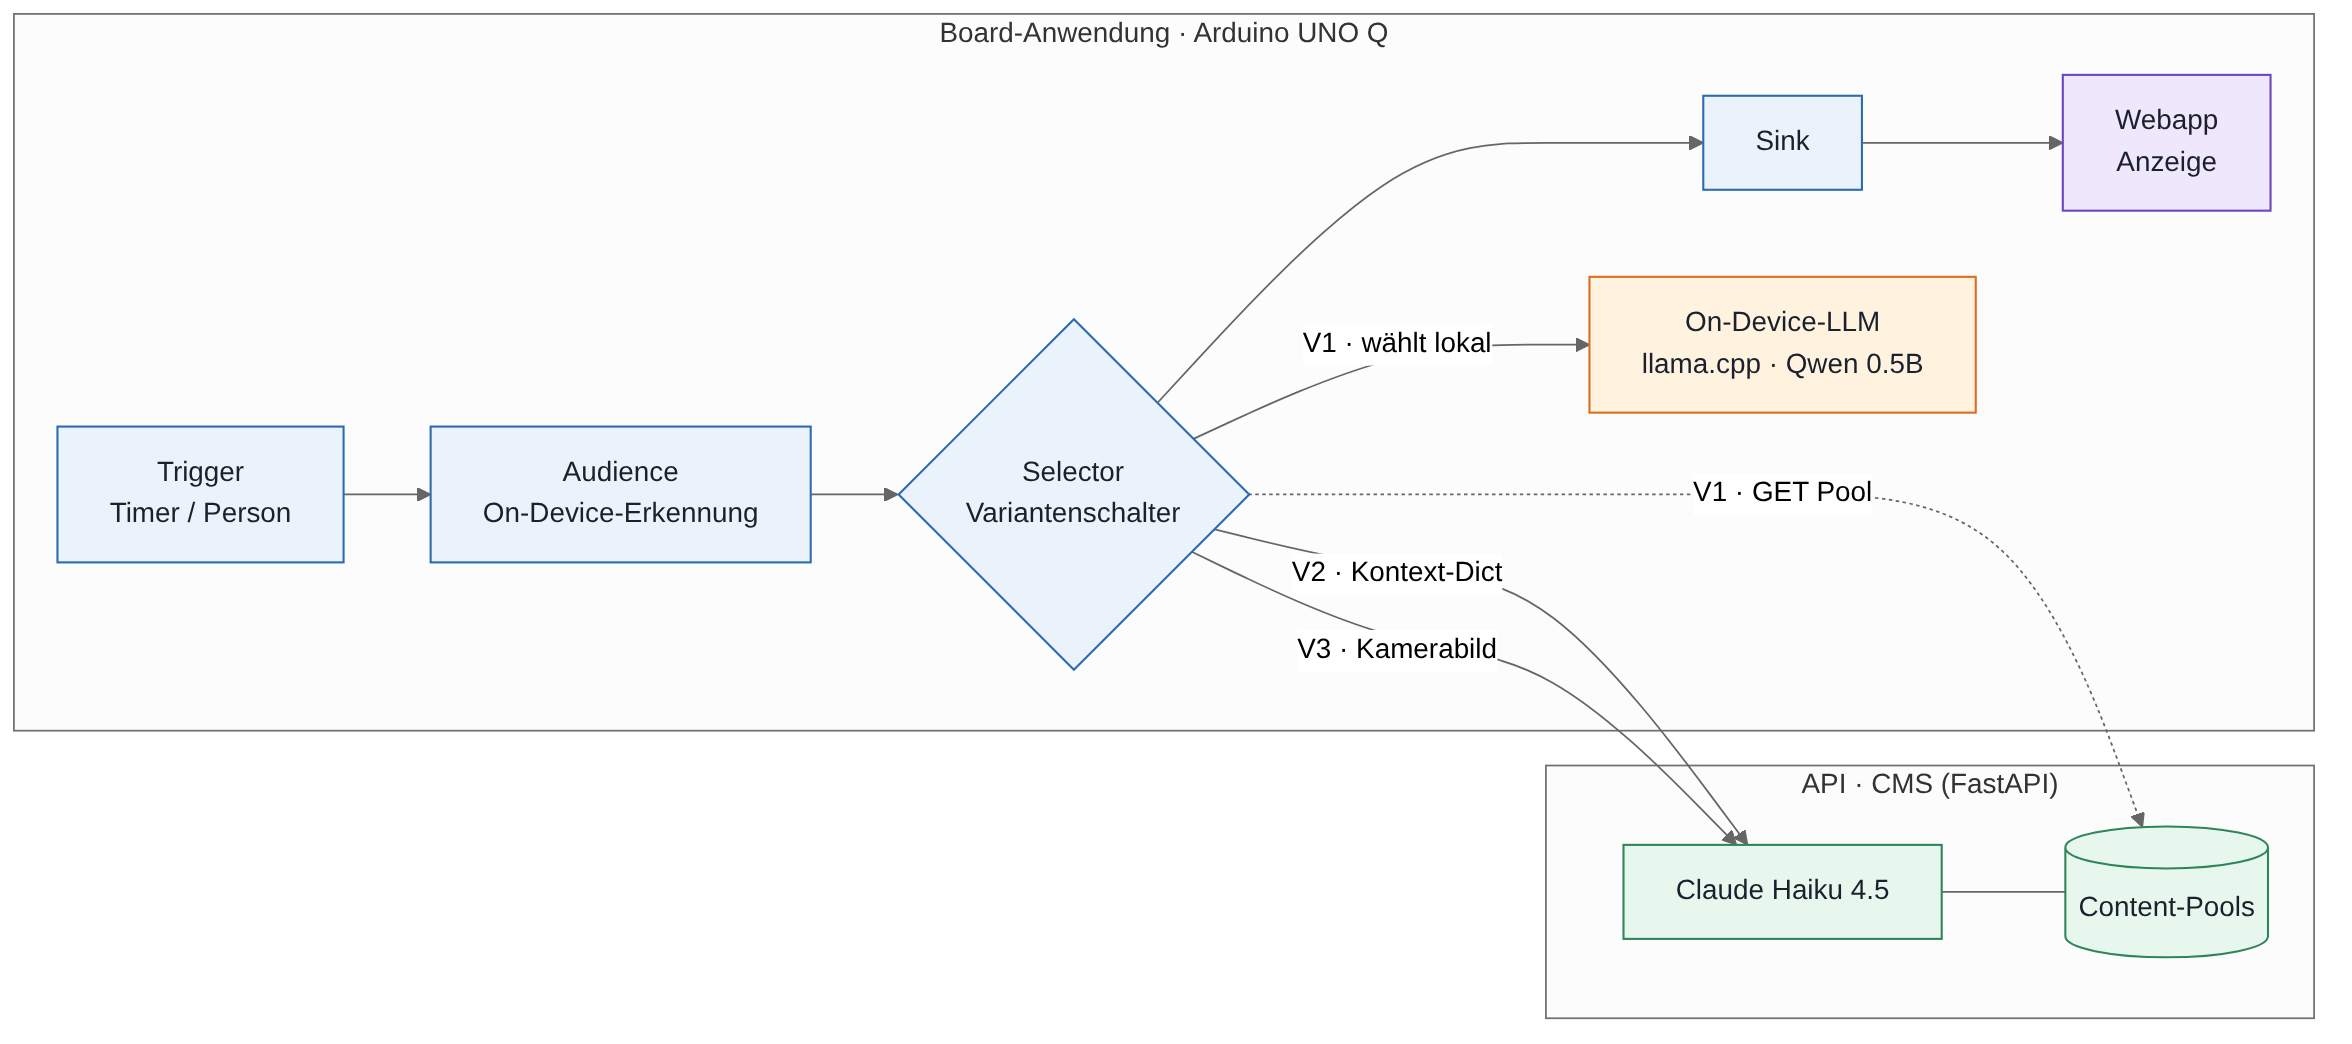
\includegraphics[width=0.9\textwidth]{figures/pipeline.png}
\caption{Die Strategy-Slot-Pipeline: vier austauschbare Stufen.}
\label{fig:pipeline}
\end{figure}

\section*{Content-Management-System}
In der Praxis verwaltet ein Content-Management-System die anzuzeigenden Inhalte und spielt sie über zeitgesteuerte Kanäle. Für die KI-Auswahl vollziehe ich einen Paradigmenwechsel: An die Stelle fester Kanäle treten \textit{Pools}, also Kandidatenmengen, aus denen pro Zyklus ein darzustellender Inhalt gewählt wird. 

Umgesetzt ist das hier als die erwähnte API-Anwendung als schlanker Platzhalter für mein Produktiv-System. Die Inhalte liegen als HTML-Dateien auf der Platte und in der Datenbank stehen nur die Metadaten. Die API drei Endpunkte bereit: \texttt{GET /pools/\{id\}} liefert den kompletten Pool, während \texttt{choose-by-context} und \texttt{choose-by-img} die Auswahl selbst treffen und nur einen Inhalt zurück senden. Für diese Auswahl in der Cloud nutze ich \texttt{Claude Haiku\,4.5} \autocite{claude}.

\section*{Zielgruppenerkennung und lokale LLMs}
Damit die \texttt{Audience}-Stufe ein belastbares Signal liefert, habe ich eine kamerabasierte Erkennung implementiert, die ausschließlich on-device arbeitet. Der Ablauf je Frame umfasst drei Schritte: Zunächst dekodiert \texttt{cv2.imdecode} das JPEG. Anschließend detektiert \texttt{YuNet} \autocite{opencvzoo} die Gesichter und liefert Crops. Schließlich schätzt ein selbst trainiertes Modell pro Gesicht das Alter und das Geschlecht. Das verwendete Modell habe ich mithilfe von \texttt{FairFace} \autocite{fairface2021} trainiert und nach ONNX exportiert. Die Einzelergebnisse aggregiere ich zu einer szenenweiten \texttt{target\_group} (bspw. \texttt{families\_with\_children} oder \texttt{seniors}).

Die Bilderkennung läuft auf dem \texttt{UNO Q} überraschend gut. \texttt{YuNet} und das \texttt{MobileNetV3-small}-Netzwerk sind kompakte für den Edge-Einsatz entworfene Technologien, sodass die Zielgruppenerkennung in wenigen Millisekunden ausführt werden kann. 

Ein On-Device-LLM läuft dagegen nicht schnell genug. Hierzu habe ich mit einer Ollama-Installation \autocite{ollama} und dem eher kleinen Modell \texttt{Qwen2.5-0.5B} experimentiert. Gemessen auf dem Board erreicht das Modell nur etwa 6 bis 7{,}5 Tokens pro Sekunde bei der Prompt-Auswertung und magere 1{,}4 bis 1{,}8 Tokens pro Sekunde bei der Generierung (rund 600\,ms je Token). Eine einzelne Auswahl dauert so leicht ein bis zwei Minuten.

\section*{Variante 1: Edge-only}
In der ersten Variante wählt das Board den Inhalt selbst, mithilfe eines On-Device-LLM. Es ruft dazu über \texttt{GET /pools/\{id\}} den gesamten Kandidaten-Pool von der API ab. Den lokal verwendeten Prompt baue ich gezielt in zwei Teilen auf: zuerst einen stabilen Teil (System-Anweisung und Kandidatenliste aus ID, Name und einer Inhalts-Beschreibung ohne der eigentlichen HTML) und den kleinen, wechselnden Kontext. Dadurch kann der Runner den Key-Value-Cache des LLM über mehrere Aufrufe hinweg wiederverwenden. Als Antwort verlange ich ausschließlich die Integer-ID des darzustellenden Inhalts. 

Der größte Aufwand steckte hier in der Optimierung der LLM-Nutzung. Anfangs benötigte eine einzelne Auswahl rund 230~Sekunden. Über mehrere Schritte habe ich die Latenz deutlich senken können, indem ich das HTML aus dem Prompt entfernt, von einer JSON- auf eine reine ID-Antwort umgestellt und das erwähnte Caching aktiviert habe. Schlussendlich dauert die erste Auswahl noch rund 96~Sekunden und jede folgende nur noch etwa 20~Sekunden. Die Auswahlqualität des 0,5B-Modells bleibt jedoch grob. In einem Test mit fünf klar gelagerten Kontexten traf es drei korrekt. Ein noch kleineres Modell würde darunter fallen, weshalb dieses Modell die sinnvolle Untergrenze markiert. 

Die Edge-only Variante erreicht damit die beste Bewertung bei Datenschutz und Kosten (keine Cloud-Aufrufe), erkauft das aber mit der im Vergleich schwächsten Korrektheit und der mit Abstand schlechtesten Performance.

\section*{Variante 2: Hybrid}
Die zweite Variante erkennt die Zielgruppe weiterhin lokal, überlässt die Auswahl aber der Cloud: Das Board sendet nur ein abstraktes Kontext-Dict an \texttt{POST /pools/\{id\}/\allowbreak choose-by-context} und \texttt{Claude} wählt daraus den passenden Inhalt aus dem Pool.

Der eigentliche Vorzug dieser Variante liegt in der Flexibilität des Übergabeformats. Das Kontext-Dict ist offen geformt, sodass sich beliebige weitere Signale (erkannte Zielgruppe, Tageszeit, künftig auch Sensordaten) ohne jeden Schnittstellenbruch einhängen lassen und direkt in den Prompt fließen. Die Architektur skaliert also mit der Menge des verfügbaren Kontexts. Ein nennenswertes Problem ergab sich dabei nicht beim Cloud-Aufruf selbst, sondern in seiner Voraussetzung. Dieser Ansatz ist immer nur so gut wie das lokale Zielgruppenerkennung. Genau das hat die oben beschriebene On-Device-Zielgruppenerkennung überhaupt erst erzwungen. 

Auf die vier Kriterien bezogen liegt diese Variante durchgängig im guten Mittelfeld. So liefert sie starken Datenschutz (das Bild wird nur lokal verarbeitet), eine gute Korrektheit dank Cloud-LLM sowie moderate Performance und Kosten, da je Auswahl nur ein kompakter Text-Prompt in die Cloud geht.

\section*{Variante 3: Cloud-only}
In der dritten Variante lädt das Board den rohen Kamera-Frame zu \texttt{POST /pools/\{id\}/\allowbreak choose-by-img} hoch und \texttt{Claude} übernimmt dann Bilderkennung sowie Auswahl in einem Schritt. Anders als die Edge- und die Hybrid-Variante führt diese Version keine Zielgruppenerkennung auf dem Board aus.

Im Test zeigte sich, dass das Rohbild mehr Information als das beabsichtigte Personen-Signal beinhaltet, sodass Szenen- und Hintergrund-Hinweise die Auswahl überlagern können. Hinzu kommt der prinzipielle Nachteil, dass das Rohbild das Gerät verlässt, was Datenschutz, Bandbreite und Netzlatenz belastet. 

Auf die vier Kriterien bezogen kehrt diese Variante also das Bild von der ersten Lösungsstrategie um. Sie liefert verlässlich die beste Korrektheit, aber die schwächsten Werte bei Datenschutz (das Rohbild verlässt das Gerät), bei den Kosten (Vision-Tokens und Bildbandbreite je Auswahl) und eine netzabhängige Performance.

\section*{Vergleich, Empfehlung und Ausblick}

\begin{table}[h]
\centering
\begin{tabularx}{\textwidth}{l *{4}{>{\centering\arraybackslash}X}}
\toprule
\textbf{Variante} & \textbf{Performance} & \textbf{Datenschutz} & \textbf{Korrektheit} & \textbf{Kosten} \\
\midrule
Edge   & schwach & sehr gut & schwach   & sehr gut \\
Hybrid & mittel                    & gut      & gut       & gut \\
Cloud  & netzabhängig              & schwach  & sehr gut  & schwach \\
\bottomrule
\end{tabularx}
\caption{Vergleich der drei Varianten entlang der vier Bewertungskriterien.}
\label{tab:variants}
\end{table}

Tabelle~\ref{tab:variants} fasst die Bewertungen zusammen. Keine der vorgeschlagenen Varianten führt auf allen vier Kriterien. Edge-only punktet bei Datenschutz und Kosten, ist aber zu langsam und ungenau. Cloud-only liefert die beste Korrektheit, gibt dafür jedoch das Kamerabild aus der Hand und verursacht die höchsten Kosten. Trotzdem verbindet der Hybrid-Ansatz die jeweiligen Stärken der anderen beiden Modelle und umgeht jeweils ihre Schwachstellen. Die Bilderkennung läuft lokal schnell und bleibt deshalb auf dem Board, sodass das Kamerabild das Gerät nie verlässt. Die für das kleine On-Device-LLM zu anspruchsvolle Auswahl wandert dagegen in die Cloud.

\end{document}
